\tikzset{every picture/.style={line width=0.75pt}} %set default line width to 0.75pt        
\centering
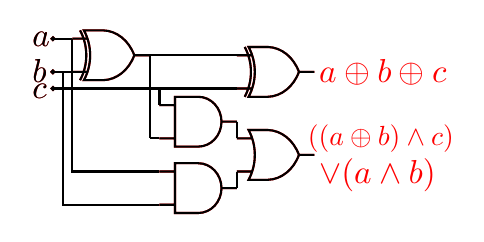
\begin{tikzpicture}[x=0.70pt,y=0.60pt,yscale=-.5,xscale=.5]
    %uncomment if require: \path (0,300); %set diagram left start at 0, and has height of 300

    \visible<1>{
        % Text Node
        \draw[red] (15,48) node [anchor=north west][inner sep=0.75pt]  [xscale=1.2,yscale=1.2] [align=left] {$a$};
        % Text Node
        \draw[red] (15,80) node [anchor=north west][inner sep=0.75pt]  [xscale=1.2,yscale=1.2] [align=left] {$b$};
        % Text Node
        \draw[red] (15,110) node [anchor=north west][inner sep=0.75pt]  [xscale=1.2,yscale=1.2] [align=left] {$c$};

        \filldraw[red] (40, 60) circle (1pt);
        \filldraw[red] (40, 100) circle (1pt);
        \filldraw[red] (40, 120) circle (1pt);
    }
    \visible<2->{
        % Text Node
        \draw (15,48) node [anchor=north west][inner sep=0.75pt]  [xscale=1.2,yscale=1.2] [align=left] {$a$};
        % Text Node
        \draw (15,80) node [anchor=north west][inner sep=0.75pt]  [xscale=1.2,yscale=1.2] [align=left] {$b$};
        % Text Node
        \draw (15,110) node [anchor=north west][inner sep=0.75pt]  [xscale=1.2,yscale=1.2] [align=left] {$c$};

        \filldraw (40, 60) circle (1pt);
        \filldraw (40, 100) circle (1pt);
        \filldraw (40, 120) circle (1pt);
    }

    \visible<2>{
        %Shape: Xor Gate [id:dp7586863585025112] 
        \draw[red]   (72,50) -- (92,50) .. controls (105.95,50.54) and (118.42,62.23) .. (124,80) .. controls (118.42,97.77) and (105.95,109.46) .. (92,110) -- (72,110) .. controls (80.57,91.44) and (80.57,68.56) .. (72,50) -- cycle (60,60) -- (76,60) (60,100) -- (76,100) (124,80) -- (140,80) (68,50) .. controls (76.57,68.56) and (76.57,91.44) .. (68,110) ;
        %Shape: Xor Gate [id:dp4857055310285392] 
        \draw[red]   (242,70) -- (262,70) .. controls (275.95,70.54) and (288.42,82.23) .. (294,100) .. controls (288.42,117.77) and (275.95,129.46) .. (262,130) -- (242,130) .. controls (250.57,111.44) and (250.57,88.56) .. (242,70) -- cycle (230,80) -- (246,80) (230,120) -- (246,120) (294,100) -- (310,100) (238,70) .. controls (246.57,88.56) and (246.57,111.44) .. (238,130) ;
        %Shape: And Gate [id:dp40243073644089766] 
        \draw[red]   (166,130) -- (190,130) .. controls (203.25,130) and (214,143.44) .. (214,160) .. controls (214,176.56) and (203.25,190) .. (190,190) -- (166,190) -- (166,130) -- cycle (150,140) -- (166,140) (150,180) -- (166,180) (214,160) -- (230,160) ;
        %Shape: And Gate [id:dp08349658070673471] 
        \draw[red]   (166,210) -- (190,210) .. controls (203.25,210) and (214,223.44) .. (214,240) .. controls (214,256.56) and (203.25,270) .. (190,270) -- (166,270) -- (166,210) -- cycle (150,220) -- (166,220) (150,260) -- (166,260) (214,240) -- (230,240) ;
        %Shape: Or Gate [id:dp5052546687696813] 
        \draw[red]   (242,170) -- (262,170) .. controls (275.95,170.54) and (288.42,182.23) .. (294,200) .. controls (288.42,217.77) and (275.95,229.46) .. (262,230) -- (242,230) .. controls (250.57,211.44) and (250.57,188.56) .. (242,170) -- cycle (230,180) -- (246,180) (230,220) -- (246,220) (294,200) -- (310,200) ;
    }
    \visible<3->{
        %Shape: Xor Gate [id:dp7586863585025112] 
        \draw   (72,50) -- (92,50) .. controls (105.95,50.54) and (118.42,62.23) .. (124,80) .. controls (118.42,97.77) and (105.95,109.46) .. (92,110) -- (72,110) .. controls (80.57,91.44) and (80.57,68.56) .. (72,50) -- cycle (60,60) -- (76,60) (60,100) -- (76,100) (124,80) -- (140,80) (68,50) .. controls (76.57,68.56) and (76.57,91.44) .. (68,110) ;
        %Shape: Xor Gate [id:dp4857055310285392] 
        \draw   (242,70) -- (262,70) .. controls (275.95,70.54) and (288.42,82.23) .. (294,100) .. controls (288.42,117.77) and (275.95,129.46) .. (262,130) -- (242,130) .. controls (250.57,111.44) and (250.57,88.56) .. (242,70) -- cycle (230,80) -- (246,80) (230,120) -- (246,120) (294,100) -- (310,100) (238,70) .. controls (246.57,88.56) and (246.57,111.44) .. (238,130) ;
        %Shape: And Gate [id:dp40243073644089766] 
        \draw   (166,130) -- (190,130) .. controls (203.25,130) and (214,143.44) .. (214,160) .. controls (214,176.56) and (203.25,190) .. (190,190) -- (166,190) -- (166,130) -- cycle (150,140) -- (166,140) (150,180) -- (166,180) (214,160) -- (230,160) ;
        %Shape: And Gate [id:dp08349658070673471] 
        \draw   (166,210) -- (190,210) .. controls (203.25,210) and (214,223.44) .. (214,240) .. controls (214,256.56) and (203.25,270) .. (190,270) -- (166,270) -- (166,210) -- cycle (150,220) -- (166,220) (150,260) -- (166,260) (214,240) -- (230,240) ;
        %Shape: Or Gate [id:dp5052546687696813] 
        \draw   (242,170) -- (262,170) .. controls (275.95,170.54) and (288.42,182.23) .. (294,200) .. controls (288.42,217.77) and (275.95,229.46) .. (262,230) -- (242,230) .. controls (250.57,211.44) and (250.57,188.56) .. (242,170) -- cycle (230,180) -- (246,180) (230,220) -- (246,220) (294,200) -- (310,200) ;
    }
    \visible<3>{
        %Straight Lines [id:da47322578625017586] 
        \draw[red]    (40,60) -- (60,60) ;
        %Straight Lines [id:da9794654949941013] 
        \draw[red]    (230,160) -- (230,180) ;
        %Straight Lines [id:da4846849793546657] 
        \draw[red]    (230,220) -- (230,240) ;
        %Straight Lines [id:da5854134933106738] 
        \draw[red]    (140,80) -- (140,120) -- (140,180) ;
        %Straight Lines [id:da21543002534508293] 
        \draw[red]    (150,180) -- (140,180) ;
        %Straight Lines [id:da2647954495406195] 
        \draw[red]    (40,120) -- (140.33,120) -- (230,120) ;
        %Straight Lines [id:da3173932178858232] 
        \draw[red]    (40,100) -- (60,100) ;
        %Straight Lines [id:da4191196124425738] 
        \draw[red]    (150,120) -- (150,140) ;
        %Straight Lines [id:da7200697769419422] 
        \draw[red]    (60,60) -- (60,220) -- (150,220) ;
        %Straight Lines [id:da6864505677890691] 
        \draw[red]    (50,100) -- (50,260) -- (150,260) ;
        %Straight Lines [id:da27064207791990746] 
        \draw[red]    (139.67,80) -- (140,80) -- (239.67,80) ;}
    \visible<4->{
        %Straight Lines [id:da47322578625017586] 
        \draw    (40,60) -- (60,60) ;
        %Straight Lines [id:da9794654949941013] 
        \draw    (230,160) -- (230,180) ;
        %Straight Lines [id:da4846849793546657] 
        \draw    (230,220) -- (230,240) ;
        %Straight Lines [id:da5854134933106738] 
        \draw    (140,80) -- (140,120) -- (140,180) ;
        %Straight Lines [id:da21543002534508293] 
        \draw    (150,180) -- (140,180) ;
        %Straight Lines [id:da2647954495406195] 
        \draw    (40,120) -- (140.33,120) -- (230,120) ;
        %Straight Lines [id:da3173932178858232] 
        \draw    (40,100) -- (60,100) ;
        %Straight Lines [id:da4191196124425738] 
        \draw    (150,120) -- (150,140) ;
        %Straight Lines [id:da7200697769419422] 
        \draw    (60,60) -- (60,220) -- (150,220) ;
        %Straight Lines [id:da6864505677890691] 
        \draw    (50,100) -- (50,260) -- (150,260) ;
        %Straight Lines [id:da27064207791990746] 
        \draw    (139.67,80) -- (140,80) -- (239.67,80) ;}

    \visible<4->{
        % Text Node
        \draw[red] (311,80) node [anchor=north west][inner sep=0.75pt]  [xscale=1.2,yscale=1.2] [align=left] {$a\oplus b\oplus c$};
        % Text Node
        \draw[red] (300,160) node [anchor=north west][inner sep=0.75pt]  [xscale=1,yscale=1] [align=left] {$(( a\oplus b) \land c)$};
        % Text Node
        \draw[red] (311,200) node [anchor=north west][inner sep=0.75pt]  [xscale=1.2,yscale=1.2] [align=left] {$ \lor ( a\land b)$};
    }


\end{tikzpicture}